\documentclass[journal]{IEEEtran}

% -----------------------------------------------------------------------------
% IEEE TIP-style manuscript draft
% Compile locally with: latexmk -pdf main.tex
% -----------------------------------------------------------------------------

\usepackage{amsmath,amssymb,amsfonts}
\usepackage{algorithm}
\usepackage{algorithmic}
\usepackage{booktabs}
\usepackage{multirow}
\usepackage{graphicx}
\usepackage{subcaption}
\usepackage{xcolor}
\usepackage{cite}
\usepackage{url}
\usepackage{bm}
\usepackage{mathtools}
\usepackage{tikz}
\usepackage{pgfplots}
\usepackage{array}
\usetikzlibrary{arrows.meta,positioning,fit,calc,shapes.geometric,shapes.misc,decorations.pathreplacing,patterns,backgrounds,shadows}
\pgfplotsset{compat=1.17}

\newcommand{\R}{\mathbb{R}}
\newcommand{\E}{\mathbb{E}}
\newcommand{\N}{\mathcal{N}}
\newcommand{\diag}{\operatorname{diag}}
\newcommand{\Tr}{\operatorname{Tr}}
\newcommand{\Norm}{\operatorname{Norm}}
\newcommand{\Corr}{\operatorname{Corr}}
\newcommand{\stopgrad}{\operatorname{stopgrad}}
\newcommand{\Charb}{\operatorname{Charb}}
\newcommand{\prox}{\operatorname{prox}}
\newcommand{\etal}{\emph{et al.}}
\newcommand{\hk}{H_{\kappa}}
\newcommand{\eps}{\varepsilon}

\definecolor{dsdbInk}{HTML}{172033}
\definecolor{dsdbBlue}{HTML}{2563EB}
\definecolor{dsdbCyan}{HTML}{06B6D4}
\definecolor{dsdbMint}{HTML}{10B981}
\definecolor{dsdbAmber}{HTML}{F59E0B}
\definecolor{dsdbRose}{HTML}{E11D48}
\definecolor{dsdbViolet}{HTML}{7C3AED}
\definecolor{dsdbPaper}{HTML}{F8FAFC}
\definecolor{dsdbLine}{HTML}{CBD5E1}

\tikzset{
    >=Latex,
    every picture/.style={font=\sffamily},
    block/.style={draw=dsdbBlue!70!black, line width=0.7pt, rounded corners=3pt, align=center, minimum height=9mm, minimum width=22mm, fill=dsdbBlue!7, text=dsdbInk, drop shadow={shadow xshift=0.7pt, shadow yshift=-0.7pt, opacity=0.18}},
    phys/.style={draw=dsdbAmber!85!black, line width=0.7pt, rounded corners=3pt, align=center, minimum height=9mm, minimum width=24mm, fill=dsdbAmber!14, text=dsdbInk, drop shadow={shadow xshift=0.7pt, shadow yshift=-0.7pt, opacity=0.18}},
    state/.style={draw=dsdbMint!70!black, line width=0.7pt, rounded corners=3pt, align=center, minimum height=9mm, minimum width=22mm, fill=dsdbMint!12, text=dsdbInk, drop shadow={shadow xshift=0.7pt, shadow yshift=-0.7pt, opacity=0.18}},
    loss/.style={draw=dsdbRose!75!black, line width=0.7pt, rounded corners=3pt, align=center, minimum height=9mm, minimum width=22mm, fill=dsdbRose!9, text=dsdbInk, drop shadow={shadow xshift=0.7pt, shadow yshift=-0.7pt, opacity=0.18}},
    panel/.style={draw=dsdbLine, rounded corners=5pt, fill=dsdbPaper, inner sep=5pt},
    tag/.style={font=\scriptsize\bfseries, text=white, rounded corners=2pt, inner xsep=4pt, inner ysep=1.5pt},
    arrow/.style={-Latex, line width=0.9pt, draw=dsdbInk!75},
    flowarrow/.style={-Latex, line width=1.15pt, draw=dsdbBlue!85!black},
    statearrow/.style={-Latex, line width=1.15pt, draw=dsdbMint!70!black},
    physarrow/.style={-Latex, line width=1.15pt, draw=dsdbAmber!90!black},
    dashedarrow/.style={-Latex, line width=0.9pt, dashed, draw=dsdbInk!55}
}

\begin{document}

\title{Degradation-State Diffusion Bridges for Metalens Photography}

\author{Xiangjun~Yin% <-this % stops a space
\thanks{Xiangjun Yin is with Affiliation Omitted for Review. E-mail: Omitted for Review.}%
\thanks{Manuscript prepared as an IEEE Transactions on Image Processing style draft.}
}

\markboth{IEEE Transactions on Image Processing,~Vol.~XX, No.~XX, 2026}%
{Yin: Degradation-State Diffusion Bridges for Metalens Photography}

\maketitle

\begin{abstract}
Metalens cameras provide an attractive route toward ultra-thin computational photography, yet their captured images are often degraded by field-dependent blur, chromatic leakage, off-axis aberrations, high-frequency ringing, and calibration drift. These degradations are spatially nonuniform and device-dependent, making metalens restoration fundamentally different from shift-invariant deblurring or generic image enhancement. Existing deterministic restoration networks tend to average ambiguous high-frequency details, while generic diffusion-based restoration methods inject globally scheduled stochasticity and may over-process reliable regions or hallucinate structures that are inconsistent with the optical measurement.

We propose a physics-anchored degradation-state diffusion bridge for metalens photography. The proposed framework first constructs a clean-domain anchor from the metalens observation using a calibrated forward operator, and estimates a fixed optical uncertainty prior that reflects spatially varying degradation strength. A dynamic degradation-state estimator then predicts the remaining local uncertainty during reverse sampling, enabling the diffusion bridge to preserve stochastic restoration capacity in severely degraded off-axis regions while suppressing unnecessary perturbations in reliable areas. In addition, an explicit metalens measurement-consistency mechanism constrains the restored image to reproduce the captured observation under the calibrated optical model. We provide a closed-form forward bridge, an analytically derived carrier target, a state-modulated reverse discretization, and a measurement projection interpreted as a proximal data-consistency step. This separation between fixed forward uncertainty and dynamic reverse-state control yields a mathematically well-defined bridge formulation and improves physical interpretability. The experimental protocol covers global fidelity, perceptual quality, off-axis restoration, measurement consistency, degradation-state diagnostics, and robustness to calibration drift; numerical entries are intentionally left blank in this manuscript template until the corresponding measurements are completed.
\end{abstract}

\begin{IEEEkeywords}
Metalens photography, computational imaging, image restoration, diffusion bridge, degradation state, measurement consistency, physics-aware image reconstruction.
\end{IEEEkeywords}

\section{Introduction}
\IEEEPARstart{M}{etalenses} have recently emerged as a promising platform for ultra-compact imaging systems. By encoding optical phase modulation into subwavelength nanostructures, metalenses can substantially reduce the thickness and weight of conventional compound optics, enabling new opportunities in mobile imaging, micro-robotics, endoscopy, AR/VR devices, and embedded vision. However, practical metalens photography remains limited by non-ideal image formation. Unlike conventional lens degradation that is often approximated as spatially invariant blur, metalens measurements exhibit strong field-dependent behavior, including off-axis blur, coma-like aberrations, chromatic leakage, reduced contrast, and high-frequency ringing. These effects vary across spatial locations, spectral channels, and device calibration states.

Such degradation makes metalens restoration a spatially nonuniform inverse problem. In the center field, the captured measurement may already contain reliable low- and mid-frequency information; near the edge field, however, the same scene structure can become severely blurred or contaminated by wavelength-dependent artifacts. A restoration method therefore cannot apply the same stochastic correction strength everywhere. Instead, it distinguishes reliable regions from uncertain regions and gradually reduces restoration uncertainty as sampling proceeds.

Existing learning-based restoration methods only partially address this challenge. Deterministic CNN or Transformer models learn a direct mapping from degraded measurements to clean images, but they typically absorb the degradation implicitly into network parameters. This strategy can achieve strong average reconstruction performance under a fixed training distribution, yet it tends to oversmooth ambiguous high-frequency details and may generalize poorly under calibration mismatch or unseen field-dependent degradation. Diffusion-based restoration methods offer stronger image priors and improved perceptual quality, but many of them rely on globally scheduled stochasticity~\cite{ho2020ddpm,song2021score,saharia2022palette,kawar2022ddrm,chung2023dps}. For metalens photography, such global stochasticity may be suboptimal: reliable regions can be unnecessarily perturbed, while severely degraded off-axis regions may still require controlled stochastic exploration. Moreover, without explicit optical measurement consistency, diffusion restoration can produce visually plausible but physically inconsistent details.

This paper addresses metalens restoration from a degradation-state perspective. Our key observation is that metalens photography requires not only a strong natural-image prior, but also an estimate of where optical uncertainty remains and when stochastic correction must be reduced. We therefore formulate restoration as a physics-anchored diffusion bridge between a clean-domain anchor and the desired clean image, rather than as unconstrained generation from noise or a direct bridge from raw degraded observations. The forward bridge uses a fixed optical uncertainty prior to preserve a valid Gaussian marginal, while the reverse process uses a dynamic degradation state to control local stochastic transport. A calibrated metalens forward operator is further incorporated into both training and sampling to enforce measurement consistency.

The main contributions are summarized as follows:
\begin{itemize}
    \item We formulate metalens photography restoration as a spatially nonuniform inverse problem with progressive uncertainty, rather than as generic deblurring or ordinary image restoration.
    \item We propose a physics-anchored degradation-state diffusion bridge that separates a clean-domain physical anchor and fixed optical uncertainty prior in the forward process from a dynamic degradation state in the reverse process, yielding a mathematically consistent and interpretable restoration framework.
    \item We derive the closed-form forward marginal, carrier target, state-modulated reverse update, and measurement-consistency projection, clarifying why the dynamic state is used only for reverse control and does not invalidate the bridge marginal.
    \item We introduce a dynamic degradation-state estimator that predicts the remaining local uncertainty during reverse sampling and explicitly modulates the bridge transport, allowing different spatial regions to receive different stochastic restoration strength.
    \item We design a metalens-specific evaluation protocol beyond global PSNR/SSIM, including edge-region fidelity, off-axis perceptual quality, re-projection measurement error, degradation-state diagnostics, calibration-drift robustness, and sampling efficiency.
\end{itemize}

\begin{figure*}[t]
\centering
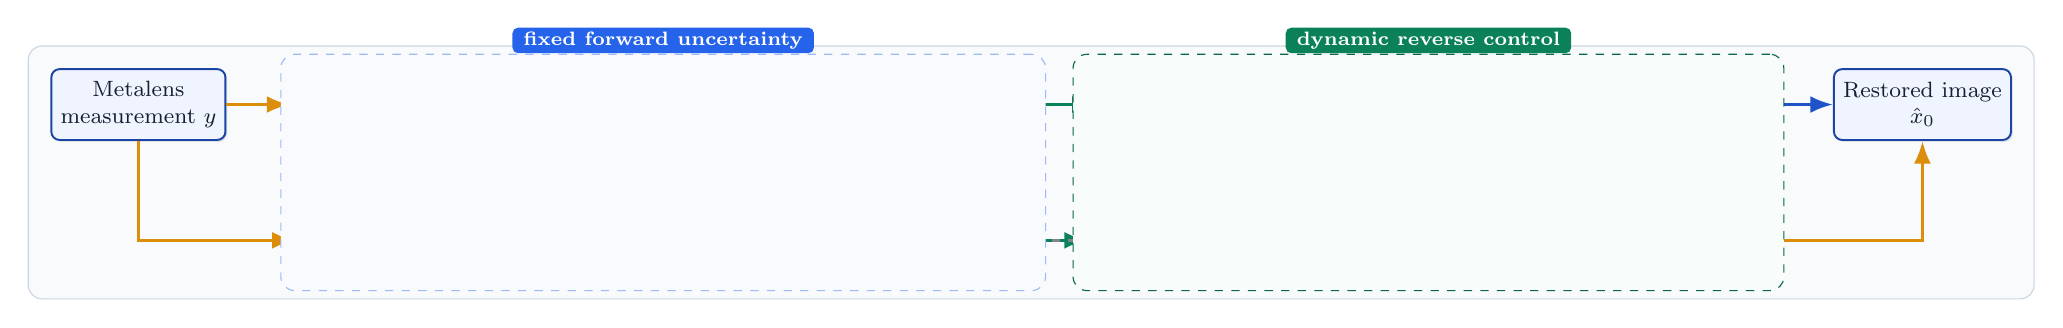
\begin{tikzpicture}[node distance=8mm and 8mm, font=\footnotesize]
    \node[block] (y) {Metalens\\measurement $y$};
    \node[phys, right=of y] (H) {Calibrated\\operator $\hk,\hk^T$};
    \node[block, right=of H] (mu) {Clean-domain\\anchor $\mu=R_0(y,\hk)$};
    \node[state, below=of H] (rho) {Optical prior\\$\rho=P_\psi(y,u,d_\kappa)$};
    \node[block, right=of mu] (xt) {Bridge state\\$x_t$};
    \node[state, right=of xt] (s) {Dynamic state\\$s_t=G_\eta(\cdot)$};
    \node[state, below=of s] (pi) {Reverse carrier\\$\Pi_t=\eps_0+\rho\odot s_t$};
    \node[block, right=of s] (F) {Carrier network\\$\hat c_t=F_\theta(\cdot)$};
    \node[block, right=of F] (update) {State-modulated\\bridge update};
    \node[loss, below=of update] (proj) {Measurement\\projection};
    \node[block, right=of update] (out) {Restored image\\$\hat x_0$};
    \begin{scope}[on background layer]
        \node[panel, fit=(y)(H)(mu)(rho)(xt)(s)(pi)(F)(update)(proj)(out), inner sep=8pt] {};
    \end{scope}
    \draw[physarrow] (y) -- (H);
    \draw[physarrow] (H) -- (mu);
    \draw[physarrow] (y) |- (rho);
    \draw[physarrow] (H) -- (rho);
    \draw[flowarrow] (mu) -- (xt);
    \draw[flowarrow] (rho) -| (xt);
    \draw[statearrow] (xt) -- (s);
    \draw[statearrow] (rho) -- (pi);
    \draw[statearrow] (s) -- (pi);
    \draw[statearrow] (s) -- (F);
    \draw[statearrow] (pi) -- (F);
    \draw[flowarrow] (F) -- (update);
    \draw[flowarrow] (update) -- (out);
    \draw[physarrow] (update) -- (proj);
    \draw[physarrow] (proj) -| (out);
    \draw[dashedarrow] (H) |- (proj);
    \node[draw=dsdbBlue!45, dashed, rounded corners=5pt, fill=dsdbBlue!3, fit=(mu)(rho)(xt), inner sep=5pt, label={[tag, fill=dsdbBlue]above:{fixed forward uncertainty}}] {};
    \node[draw=dsdbMint!55!black, dashed, rounded corners=5pt, fill=dsdbMint!3, fit=(s)(pi)(F)(update), inner sep=5pt, label={[tag, fill=dsdbMint!70!black]above:{dynamic reverse control}}] {};
\end{tikzpicture}
\caption{Overview of the proposed physics-anchored degradation-state diffusion bridge. The metalens operator first provides a clean-domain anchor and optical uncertainty prior. The fixed prior $\rho$ defines the forward bridge marginal, while the dynamic state $s_t$ modulates only the reverse stochastic transport through $\Pi_t$. A measurement-consistency projection using $\hk$ and $\hk^T$ suppresses hallucinated details.}
\label{fig:overview}
\end{figure*}

\section{Related Work}
\subsection{Computational Metalens Imaging}
Metalenses enable compact optical systems by replacing bulky refractive elements with planar nanostructures. However, practical metalens imaging is affected by spatially varying point spread functions, chromatic response mismatch, field-dependent resolution, and fabrication-induced deviations. Computational reconstruction is therefore essential for high-quality metalens photography. Existing correction methods include calibrated deconvolution, learned restoration, and hybrid optical-computational pipelines. Their performance depends strongly on how accurately the degradation is represented and how robustly the reconstruction handles calibration mismatch.

\subsection{Image Restoration Under Spatially Variant Degradation}
Classical restoration methods often assume a known or estimated degradation operator. When the degradation is spatially variant, the inverse problem becomes ill-conditioned and region-dependent. Deep neural networks can learn powerful priors, but they often treat degradation as implicit training bias. This can limit interpretability and robustness under unseen optical states. For metalens photography, the degradation is tied to field position and spectral response, requiring restoration strategies that explicitly account for spatially varying uncertainty.

\subsection{Diffusion Models for Inverse Problems}
Diffusion models provide strong natural-image priors and have been applied to inverse imaging tasks through denoising diffusion, score-based modeling, conditional image-to-image generation, posterior sampling, and plug-and-play measurement guidance~\cite{ho2020ddpm,song2021score,saharia2022palette,kawar2022ddrm,chung2023dps}. Although these methods can improve perceptual quality, they may introduce hallucinated details when measurement consistency is weak. In metalens photography, this risk is amplified because optical degradation removes or entangles high-frequency information in a spatially nonuniform manner.

\subsection{Diffusion Bridges and State-Guided Restoration}
Diffusion bridges model stochastic transport between two endpoint distributions or between an observation and a target image manifold. Compared with unconditional diffusion from pure noise, a bridge formulation is more suitable for restoration because the process is anchored by the observation. However, existing bridge-based restoration methods often use static residual modeling or global schedules. We instead introduce a degradation state that evolves during reverse sampling and controls local stochasticity according to remaining optical uncertainty.

\section{Problem Formulation}
Let $x_0 \in \R^{H\times W\times C}$ denote the desired clean image and $y \in \R^{H\times W\times C}$ denote the observed metalens measurement. We model the metalens image formation process as
\begin{equation}
    y = \hk(x_0) + n,
    \label{eq:forward_basic}
\end{equation}
where $\hk$ is a calibrated metalens forward operator parameterized by calibration state $\kappa$, and $n$ denotes measurement noise. Unlike shift-invariant blur operators, $\hk$ is spatially variant and may incorporate field-dependent PSFs, channel mixing, spectral leakage, and sensor response.

A more explicit form can be written as
\begin{equation}
    y_c(p)=S_c\left\{\sum_{\lambda}\int h_{\kappa,p,\lambda}(q)x_{\lambda}(p-q)dq\right\}+n_c(p),
    \label{eq:forward_explicit}
\end{equation}
where $p$ is the spatial position, $c$ indexes the sensor channel, $h_{\kappa,p,\lambda}$ denotes the local PSF at field position $p$ and wavelength $\lambda$, and $S_c$ represents the sensor spectral response or RGB channel mixing. In implementation, $\hk$ can be approximated by a PSF bank with spatial interpolation and optional RGB channel mixing.

The restoration task is to estimate
\begin{equation}
    \hat{x}_0 = \mathcal{R}(y,\hk)
\end{equation}
such that $\hat{x}_0$ is perceptually plausible, structurally faithful, and consistent with the measurement $y$ under $\hk$.

A central difficulty is that the uncertainty of this inverse problem is not uniform across the image. Let $u$ denote the field-coordinate map. Regions with large field radius, anisotropic PSF, low MTF, or strong chromatic shift are expected to have higher restoration uncertainty. We therefore introduce two complementary uncertainty variables: a fixed optical uncertainty prior $\rho$, used in the forward bridge, and a dynamic degradation state $s_t$, used only in reverse sampling. This separation is essential. The forward process must remain analytically tractable and free of self-referential dependence on $x_t$, while the reverse process remains adaptive to the current sampling state.

\section{Physics-Anchored Degradation-State Diffusion Bridge}
\subsection{Clean-Domain Anchor}
Directly anchoring a diffusion bridge to the raw metalens measurement $y$ causes a domain mismatch because $y$ lies in the degraded measurement domain, whereas $x_0$ lies in the clean image domain. We therefore construct a clean-domain anchor
\begin{equation}
    \mu = R_0(y,\hk),
    \label{eq:anchor}
\end{equation}
where $R_0$ is a calibration-aware initial reconstruction module. It can be implemented using physics-guided deconvolution, an ADMM/Wiener reconstruction, a lightweight neural initializer, or a hybrid deconvolution-plus-refinement module. The role of $\mu$ is not to solve the entire restoration problem, but to provide a physically meaningful clean-domain endpoint around which the diffusion bridge models residual uncertainty. This design avoids forcing the bridge to connect heterogeneous domains and reduces the burden on the stochastic restoration process.

\subsection{Optical Uncertainty Prior}
We estimate a fixed spatial uncertainty prior
\begin{equation}
    \rho = P_{\psi}(y,u,d_{\kappa}),
    \label{eq:rho}
\end{equation}
where $P_{\psi}$ is an optical-prior estimator and $d_{\kappa}$ denotes physical descriptors derived from the metalens calibration, such as PSF FWHM, MTF50, PSF anisotropy, field radius, field angle, Strehl ratio, or chromatic centroid shift. The prior $\rho$ reflects where the optical inverse problem is intrinsically less reliable. It is fixed for a given observation during forward bridge construction and does not depend on the intermediate sample $x_t$.

\subsection{Forward Bridge}
Given clean target $x_0$, clean-domain anchor $\mu$, and uncertainty prior $\rho$, the forward bridge is defined as
\begin{equation}
    q(x_t|x_0,\mu,\rho)=\N\left(\mu+\Theta_t(x_0-\mu),\Sigma_t^2\diag(\rho^2)\right),
    \label{eq:forward_bridge}
\end{equation}
or equivalently,
\begin{equation}
    x_t=\mu+\Theta_t(x_0-\mu)+\Sigma_t\rho\odot\epsilon,
    \quad \epsilon\sim\N(0,I).
    \label{eq:forward_sample}
\end{equation}
We use the reverse-time convention $t=T,\ldots,0$, with $\Theta_0=1$ and $\Sigma_0=0$ at the clean endpoint, and $\Theta_T\approx0$ with the largest $\Sigma_T$ near the anchor/noisy endpoint. Here, $\Theta_t$ controls the deterministic residual interpolation from $x_0-\mu$ to zero, $\Sigma_t$ controls the global noise schedule, and $\rho$ modulates spatial uncertainty. A larger $\rho$ allows stronger corruption in optically unreliable regions, while a smaller $\rho$ preserves reliable regions closer to the clean-domain anchor.

The carrier target is obtained from the forward sampling equation:
\begin{equation}
    c_t^{*}=\epsilon=\frac{x_t-\mu-\Theta_t(x_0-\mu)}{\Sigma_t\rho+\eps_0},
    \label{eq:carrier_target}
\end{equation}
where $\eps_0$ is a small constant for numerical stability.

\subsection{Dynamic Degradation State}
The dynamic degradation state $s_t$ represents the remaining local uncertainty during reverse sampling. Unlike $\rho$, it is not part of the forward marginal. Instead, it serves as an adaptive reverse-control variable:
\begin{equation}
    s_t=\sigma\left(G_{\eta}\left(x_t,\mu,y,\rho,u,e_t,r_t\right)\right),
    \label{eq:state}
\end{equation}
where $G_{\eta}$ is a state estimator, $\sigma(\cdot)$ is a sigmoid function, $e_t$ is the time embedding, and $r_t$ denotes residual cues such as $|x_t-\mu|$, $\hk(x_t)-y$, local gradient mismatch, or Laplacian mismatch. The local reverse uncertainty carrier is then defined as
\begin{equation}
    \Pi_t=\eps_0+\rho\odot s_t.
    \label{eq:pi}
\end{equation}
This variable explicitly enters the reverse update. In reliable regions, $s_t$ is expected to decay rapidly, reducing unnecessary stochasticity. In off-axis or chromatically degraded regions, $s_t$ may remain higher for more sampling steps, allowing controlled restoration of uncertain high-frequency content.

\subsection{State-Modulated Reverse Bridge}
The carrier network predicts
\begin{equation}
    \hat{c}_t=F_{\theta}(x_t,\mu,y,\Pi_t,u,t),
    \label{eq:carrier_pred}
\end{equation}
where $F_{\theta}$ can be implemented with a U-Net, Restormer-style blocks, or a hybrid CNN-Transformer architecture. A state-modulated bridge update can be written as
\begin{equation}
    \tilde{x}_{t-1}=\mu+\frac{\Theta_{t-1}}{\Theta_t}(x_t-\mu)-B_t(\Pi_t,\Pi_{t-1})\odot\hat{c}_t,
    \label{eq:reverse_update}
\end{equation}
with
\begin{equation}
    B_t(\Pi_t,\Pi_{t-1})=\frac{\Theta_{t-1}}{\Theta_t}\Sigma_t\Pi_t-\Sigma_{t-1}\Pi_{t-1}.
    \label{eq:b_t}
\end{equation}
For stable implementation, one may use the discretized approximation
\begin{equation}
    \tilde{x}_{t-1}=\mu+\frac{\Theta_{t-1}}{\Theta_t}(x_t-\mu)-\beta_t\Pi_t\odot\hat{c}_t,
    \label{eq:reverse_update_approx}
\end{equation}
where $\beta_t$ is a precomputed scalar determined by the sampling schedule. This approximation can be interpreted as a stable discretization of the state-modulated bridge transport.

\subsection{Measurement-Consistency Projection}
To reduce hallucination and ensure physical consistency, the restored sample is corrected using the metalens forward operator:
\begin{equation}
    x_{t-1}=\tilde{x}_{t-1}-\gamma_t\hk^T W^T W\left(\hk(\tilde{x}_{t-1})-y\right),
    \label{eq:projection}
\end{equation}
where $\hk^T$ denotes the adjoint or back-projection operator for a linear operator, or the Jacobian adjoint for a differentiable nonlinear operator; $\gamma_t$ is a step-dependent correction strength. This projection encourages the restored image to remain consistent with the captured metalens measurement. The corresponding measurement loss is
\begin{equation}
    \mathcal{L}_{\mathrm{meas}}=\left\|W\odot\left(\hk(\hat{x}_0)-y\right)\right\|_1,
    \label{eq:loss_meas}
\end{equation}
where $W$ is a reliability mask that can down-weight saturated, underexposed, noisy, or misregistered regions.

\begin{figure*}[t]
\centering
\begin{subfigure}[t]{0.31\textwidth}
\centering
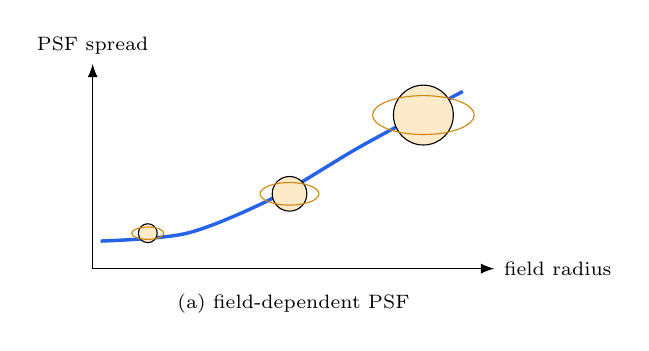
\begin{tikzpicture}[font=\scriptsize]
\draw[->] (0,0) -- (5.1,0) node[right] {field radius};
\draw[->] (0,0) -- (0,2.6) node[above] {PSF spread};
\draw[line width=1.25pt, dsdbBlue] plot[smooth] coordinates {(0.1,0.35) (1.2,0.45) (2.3,0.9) (3.4,1.55) (4.7,2.25)};
\foreach \x/\y/\r in {0.7/0.45/0.12,2.5/0.95/0.22,4.2/1.95/0.38}{
  \draw[fill=dsdbAmber!22] (\x,\y) circle (\r);
  \draw[dsdbAmber!85!black] (\x,\y) ellipse ({1.7*\r} and {0.65*\r});
}
\node at (2.55,-0.45) {(a) field-dependent PSF};
\end{tikzpicture}
\end{subfigure}
\begin{subfigure}[t]{0.34\textwidth}
\centering
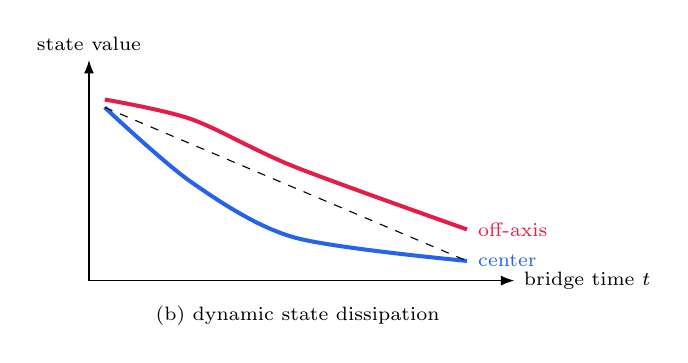
\begin{tikzpicture}[font=\scriptsize]
\draw[->] (0,0) -- (5.4,0) node[right] {bridge time $t$};
\draw[->] (0,0) -- (0,2.8) node[above] {state value};
\draw[line width=1.45pt, dsdbBlue] plot[smooth] coordinates {(0.2,2.2) (1.3,1.25) (2.6,0.55) (4.8,0.25)} node[right] {center};
\draw[line width=1.45pt, dsdbRose] plot[smooth] coordinates {(0.2,2.3) (1.3,2.05) (2.6,1.45) (4.8,0.65)} node[right] {off-axis};
\draw[dashed] (0.2,2.2) -- (4.8,0.25);
\node at (2.65,-0.45) {(b) dynamic state dissipation};
\end{tikzpicture}
\end{subfigure}
\begin{subfigure}[t]{0.31\textwidth}
\centering
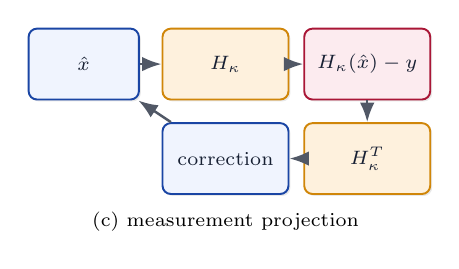
\begin{tikzpicture}[font=\scriptsize]
\node[block, minimum width=14mm] (x) at (0,0) {$\hat x$};
\node[phys, minimum width=16mm] (h) at (1.8,0) {$\hk$};
\node[loss, minimum width=16mm] (r) at (3.6,0) {$\hk(\hat x)-y$};
\node[phys, minimum width=16mm] (ht) at (3.6,-1.2) {$\hk^T$};
\node[block, minimum width=16mm] (corr) at (1.8,-1.2) {correction};
\draw[arrow] (x)--(h); \draw[arrow] (h)--(r); \draw[arrow] (r)--(ht); \draw[arrow] (ht)--(corr); \draw[arrow] (corr)--(x);
\node at (1.8,-2.0) {(c) measurement projection};
\end{tikzpicture}
\end{subfigure}
\caption{Conceptual illustrations used throughout the method. (a) Metalens degradation grows with field radius and is represented by a spatial optical prior. (b) The dynamic state decays faster in reliable center regions and remains higher in off-axis regions. (c) The projection step uses the metalens operator to reduce measurement inconsistency. These drawings are vector TikZ figures and can be replaced by experiment-derived visualizations.}
\label{fig:concepts}
\end{figure*}

\section{Theoretical Analysis}

\begin{figure*}[t]
\centering
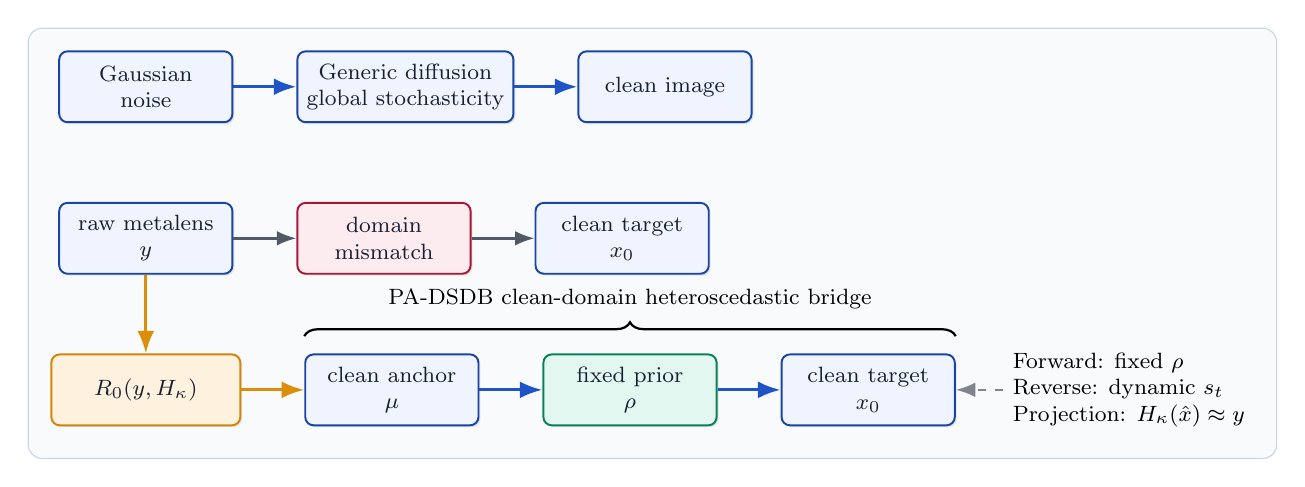
\begin{tikzpicture}[font=\footnotesize, node distance=7mm and 8mm]
\node[block] (noise) {Gaussian\\noise};
\node[block, right=of noise] (diff) {Generic diffusion\\global stochasticity};
\node[block, right=of diff] (clean1) {clean image};
\draw[flowarrow] (noise)--(diff); \draw[flowarrow] (diff)--(clean1);
\node[block, below=10mm of noise] (raw) {raw metalens\\$y$};
\node[loss, right=of raw] (mismatch) {domain\\mismatch};
\node[block, right=of mismatch] (clean2) {clean target\\$x_0$};
\draw[arrow] (raw)--(mismatch); \draw[arrow] (mismatch)--(clean2);
\node[phys, below=10mm of raw] (op) {$R_0(y,\hk)$};
\node[block, right=of op] (anchor) {clean anchor\\$\mu$};
\node[state, right=of anchor] (prior) {fixed prior\\$\rho$};
\node[block, right=of prior] (clean3) {clean target\\$x_0$};
\draw[physarrow] (raw)--(op); \draw[physarrow] (op)--(anchor); \draw[flowarrow] (anchor)--(prior); \draw[flowarrow] (prior)--(clean3);
\draw[decorate, decoration={brace, amplitude=5pt}, thick] ($(anchor.north west)+(0,0.22)$) -- node[above=6pt] {PA-DSDB clean-domain heteroscedastic bridge} ($(clean3.north east)+(0,0.22)$);
\node[align=left, right=6mm of clean3] (note) {Forward: fixed $\rho$\\Reverse: dynamic $s_t$\\Projection: $\hk(\hat x)\approx y$};
\draw[dashedarrow] (note.west)--(clean3.east);
\begin{scope}[on background layer]
    \node[panel, fit=(noise)(diff)(clean1)(raw)(mismatch)(clean2)(op)(anchor)(prior)(clean3)(note), inner sep=8pt] {};
\end{scope}
\end{tikzpicture}
\caption{Bridge geometry. Generic diffusion starts from noise and uses global stochasticity, while a direct raw-observation bridge suffers from domain mismatch because $y$ lies in the degraded measurement domain. PA-DSDB first maps $y$ to a clean-domain anchor $\mu$ and defines a heteroscedastic bridge between $\mu$ and $x_0$ using fixed optical uncertainty $\rho$; the dynamic state $s_t$ is reserved for reverse control.}
\label{fig:bridge_geometry}
\end{figure*}

This section gives the mathematical support for the proposed design. The goal is not to claim an exact physical posterior solver, but to show that each component has a well-defined role and that the dynamic state does not break the forward bridge marginal.

\subsection{Validity of the Forward Marginal}
\textbf{Proposition 1.} If $\rho$ is fixed with respect to $x_t$ for a given pair $(x_0,y)$, the random variable in~\eqref{eq:forward_sample} has the Gaussian marginal in~\eqref{eq:forward_bridge}.

\emph{Proof.} The only random term in~\eqref{eq:forward_sample} is $\Sigma_t\rho\odot\epsilon$. Since $\epsilon\sim\N(0,I)$ and multiplication by the diagonal matrix $\Sigma_t\diag(\rho)$ is an affine transformation of a Gaussian variable,
\begin{equation}
    \Sigma_t\diag(\rho)\epsilon \sim \N\left(0,\Sigma_t^2\diag(\rho^2)\right).
\end{equation}
Adding the deterministic mean $\mu+\Theta_t(x_0-\mu)$ yields~\eqref{eq:forward_bridge}. \hfill$\square$

This proposition motivates the separation between $\rho$ and $s_t$. If a sample-dependent state were inserted into the forward variance, the marginal would no longer be the stated closed-form Gaussian unless an additional conditional model were specified.

\subsection{Carrier Target and Score Equivalence}
The carrier target in~\eqref{eq:carrier_target} is the standardized residual of the bridge. Under the Gaussian marginal in~\eqref{eq:forward_bridge}, the conditional score is
\begin{equation}
    \nabla_{x_t}\log q(x_t|x_0,\mu,\rho)
    =-\frac{x_t-\mu-\Theta_t(x_0-\mu)}{\Sigma_t^2\rho^2+\eps_0^2}.
    \label{eq:score_bridge}
\end{equation}
Combining~\eqref{eq:carrier_target} and~\eqref{eq:score_bridge} gives
\begin{equation}
    \nabla_{x_t}\log q(x_t|x_0,\mu,\rho)
    \approx -\frac{c_t^*}{\Sigma_t\rho+\eps_0}.
\end{equation}
Thus, predicting $c_t^*$ is equivalent to predicting a scaled bridge score. This parameterization is numerically convenient because the target is approximately standard normal and spatially normalized by the optical uncertainty prior.

\subsection{Derivation of the State-Modulated Reverse Update}
Ignoring measurement projection, a clean estimate from the carrier prediction can be written as
\begin{equation}
    \hat{x}_{0|t}=\mu+\frac{x_t-\mu-\Sigma_t\Pi_t\odot\hat c_t}{\Theta_t}.
    \label{eq:x0_est}
\end{equation}
When $\Pi_t=\Pi_{t-1}=\rho$, a deterministic bridge step evaluates the previous state using the same clean estimate:
\begin{equation}
    \tilde{x}_{t-1}=\mu+\Theta_{t-1}(\hat{x}_{0|t}-\mu)+\Sigma_{t-1}\Pi_{t-1}\odot\hat c_t.
\end{equation}
Substituting~\eqref{eq:x0_est} into the above equation yields
\begin{equation}
\begin{split}
    \tilde{x}_{t-1}={}&\mu+\frac{\Theta_{t-1}}{\Theta_t}(x_t-\mu) \\
    &-\left(\frac{\Theta_{t-1}}{\Theta_t}\Sigma_t\Pi_t-\Sigma_{t-1}\Pi_{t-1}\right)\odot\hat c_t,
\end{split}
\end{equation}
which gives~\eqref{eq:reverse_update}. When $\Pi_t=\Pi_{t-1}=\rho$, the update reduces to the deterministic transport implied by the forward bridge. When $\Pi_t=\eps_0+\rho\odot s_t$, the update is interpreted as a state-controlled reverse discretization rather than an exact posterior transition. This distinction is important: the carrier target is normalized by the fixed forward prior $\rho$, while $\Pi_t$ adaptively rescales the reverse transport magnitude according to remaining local uncertainty. In implementation, we use the stable one-step approximation in~\eqref{eq:reverse_update_approx}, which depends only on the current $\Pi_t$ and avoids predicting $\Pi_{t-1}$.

\subsection{Measurement Projection as Data-Consistency Descent}
Consider the weighted quadratic measurement energy
\begin{equation}
    \mathcal{D}(x)=\frac{1}{2}\|W\odot(\hk(x)-y)\|_2^2.
\end{equation}
If $\hk$ is linear, its gradient is
\begin{equation}
    \nabla_x\mathcal{D}(x)=\hk^T W^T W(\hk(x)-y).
\end{equation}
For a differentiable nonlinear operator, $\hk^T$ is replaced by the Jacobian adjoint $J_{\hk}(x)^T$. Therefore,~\eqref{eq:projection} is implemented as a first-order data-consistency step; the robust $L_1$ term in~\eqref{eq:loss_meas} is used for training, while the local quadratic form provides a stable sampling correction. For a linear operator, if $0<\gamma_t<2/\|\hk^T W^T W\hk\|_2$, the step is non-expansive with respect to the quadratic data term. This provides a stable interpretation of the projection and clarifies why it reduces hallucination: details that cannot reproduce the measured metalens observation are penalized by the forward model.

\subsection{State Regularization and Interpretability}
Let $E_t=|\hat{x}_{0|t}-x_0|$ denote paired reconstruction error, or let $M_t=|\hk(\hat{x}_{0|t})-y|$ denote weak measurement residual. The proposed state alignment loss encourages
\begin{equation}
    s_t(p) \propto E_t(p) \quad \text{or} \quad s_t(p) \propto M_t(p),
\end{equation}
while the dissipation loss encourages a progressive reduction of uncertainty along the reverse trajectory. These constraints make $s_t$ experimentally falsifiable: a meaningful state correlates with error/residual maps, decays over sampling, and responds to increased optical degradation or calibration drift.

\section{Network Architecture and Implementation}
\subsection{Module Design}
The proposed system contains five modules. The anchor generator $R_0$ produces the clean-domain initialization $\mu$ from $y$ and $\hk$. The optical prior estimator $P_\psi$ predicts $\rho$ from observation cues, field coordinates, and physical descriptors. The state estimator $G_\eta$ predicts $s_t$ from the current bridge sample, anchor, measurement, residual cues, and time embedding. The carrier network $F_\theta$ predicts $\hat c_t$ under state-modulated conditioning. Finally, the measurement projector applies one or a few gradient steps using $\hk$ and $\hk^T$.

\begin{table*}[t]
\centering
\caption{Module configuration. The table is intended as a reproducible implementation specification and can be adapted to the final codebase.}
\label{tab:modules}
\begin{tabular}{p{0.18\textwidth}p{0.25\textwidth}p{0.27\textwidth}p{0.2\textwidth}}
\toprule
Module & Input & Suggested structure & Output / role \\
\midrule
Anchor generator $R_0$ & $y$, optional PSF descriptors & Wiener/ADMM initialization followed by shallow U-Net, or a lightweight Restormer draft & Clean-domain anchor $\mu$ \\
Optical prior $P_\psi$ & $y,u,d_\kappa$ & 3-level CNN with coordinate encoding & Fixed uncertainty prior $\rho\in[\rho_{\min},\rho_{\max}]$ \\
State estimator $G_\eta$ & $x_t,\mu,y,\rho,r_t,e_t$ & Lightweight CNN with FiLM/SFT time modulation & Dynamic state $s_t\in[0,1]$ \\
Carrier network $F_\theta$ & $x_t,\mu,y,\Pi_t,u,t$ & U-Net / Restormer hybrid with residual blocks & Carrier prediction $\hat c_t$ \\
Projector & $\tilde x_{t-1},y,\hk$ & One-step gradient or proximal correction & Measurement-consistent $x_{t-1}$ \\
\bottomrule
\end{tabular}
\end{table*}


\begin{figure*}[t]
\centering
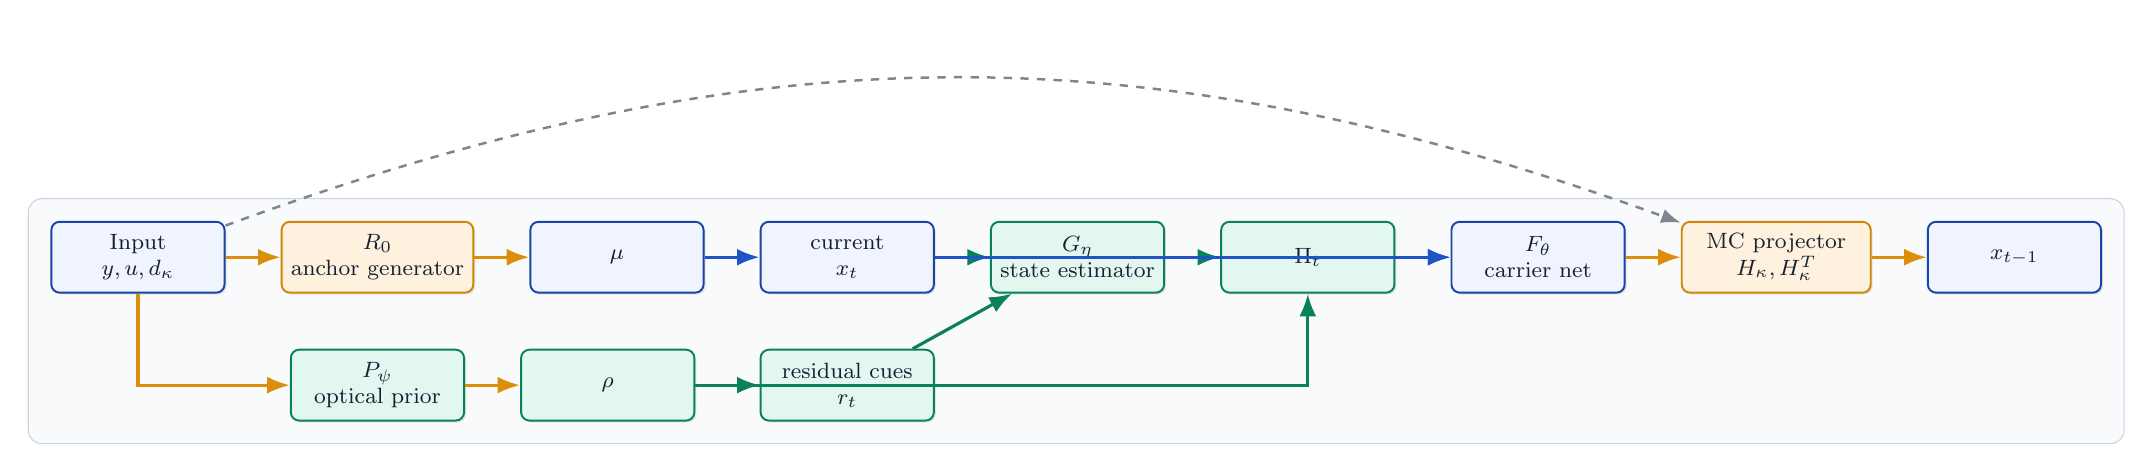
\begin{tikzpicture}[font=\footnotesize, node distance=7mm and 7mm]
\node[block] (input) {Input\\$y,u,d_\kappa$};
\node[phys, right=of input] (r0) {$R_0$\\anchor generator};
\node[state, below=of r0] (p) {$P_\psi$\\optical prior};
\node[block, right=of r0] (mu) {$\mu$};
\node[state, right=of p] (rho) {$\rho$};
\node[block, right=of mu] (sample) {current\\$x_t$};
\node[state, below=of sample] (res) {residual cues\\$r_t$};
\node[state, right=of sample] (g) {$G_\eta$\\state estimator};
\node[state, right=of g] (pi) {$\Pi_t$};
\node[block, right=of pi] (f) {$F_\theta$\\carrier net};
\node[phys, right=of f] (proj) {MC projector\\$\hk,\hk^T$};
\node[block, right=of proj] (out) {$x_{t-1}$};
\begin{scope}[on background layer]
    \node[panel, fit=(input)(r0)(p)(mu)(rho)(sample)(res)(g)(pi)(f)(proj)(out), inner sep=8pt] {};
\end{scope}
\draw[physarrow] (input)--(r0); \draw[physarrow] (input)|-(p); \draw[physarrow] (r0)--(mu); \draw[physarrow] (p)--(rho);
\draw[flowarrow] (mu)--(sample); \draw[statearrow] (rho)--(res); \draw[statearrow] (sample)--(g); \draw[statearrow] (res)--(g); \draw[statearrow] (g)--(pi); \draw[statearrow] (rho)-|(pi);
\draw[flowarrow] (pi)--(f); \draw[flowarrow] (sample)--(f); \draw[physarrow] (f)--(proj); \draw[physarrow] (proj)--(out);
\draw[dashedarrow] (input) to[bend left=20] (proj);
\end{tikzpicture}
\caption{Network architecture at one reverse step. The anchor generator and optical-prior estimator are observation-level modules. The state estimator and carrier network operate at each reverse step, using residual cues and the local carrier $\Pi_t$ to control the state-modulated transport before measurement-consistency projection.}
\label{fig:architecture}
\end{figure*}

\subsection{Cue Construction}
The state estimator is designed not to rely only on color differences such as $|R-G|$ and $|B-G|$, because true color edges may be confused with chromatic degradation. We divide cues into physical, observation, dynamic, and temporal cues. Physical cues include PSF FWHM, MTF50, MTF10, Strehl ratio, PSF anisotropy, chromatic centroid shift, field radius, and field angle. Observation cues include local contrast, saturation masks, noise estimates, edge confidence, and color residual consistency. Dynamic cues include $|x_t-\mu|$, $|\hk(x_t)-y|$, gradient mismatch, Laplacian mismatch, and feature residuals. Temporal cues use sinusoidal or learned embeddings of $t$.

\section{Training Objective}
The carrier loss is
\begin{equation}
    \mathcal{L}_{\mathrm{carrier}}=\E\left[\left\|F_{\theta}(x_t,\mu,y,\Pi_t,u,t)-c_t^{*}\right\|_1\right].
    \label{eq:loss_carrier}
\end{equation}
The reconstruction loss is
\begin{equation}
    \mathcal{L}_{\mathrm{rec}}=\|\hat{x}_0-x_0\|_1+\lambda_g\Charb\left(\nabla\hat{x}_0-\nabla x_0\right).
    \label{eq:loss_rec}
\end{equation}
To improve perceptual quality, a feature-level loss can be used:
\begin{equation}
    \mathcal{L}_{\mathrm{perc}}=\|\phi(\hat{x}_0)-\phi(x_0)\|_1,
    \label{eq:loss_perc}
\end{equation}
where $\phi(\cdot)$ is a pretrained perceptual feature extractor.

The optical prior can be supervised by a target uncertainty map
\begin{equation}
    \rho^{*}=\Norm\left(\alpha|x_0-\mu|+\beta M_{\mathrm{edge}}(u)+\chi D_{\kappa}(u)\right),
    \label{eq:rho_target}
\end{equation}
where $D_{\kappa}(u)$ is a physical degradation descriptor derived from PSF/MTF statistics. The prior loss is
\begin{equation}
    \mathcal{L}_{\mathrm{prior}}=\|\rho-\rho^{*}\|_1.
    \label{eq:loss_prior}
\end{equation}

To prevent the degradation state from degenerating into an unconstrained attention map, we regularize it using error alignment and temporal dissipation. Given an intermediate clean estimate $\hat{x}_{0|t}$, define
\begin{equation}
    E_t=|\hat{x}_{0|t}-x_0|
\end{equation}
for paired data, or
\begin{equation}
    M_t=|\hk(\hat{x}_{0|t})-y|
\end{equation}
for weakly supervised real data. We define a unified uncertainty target
\begin{equation}
U_t=\begin{cases}
E_t, & \text{paired training data},\\
M_t, & \text{weakly supervised real data}.
\end{cases}
\end{equation}
The alignment loss can be written as
\begin{equation}
    \mathcal{L}_{\mathrm{align}}=\left\|\Norm(s_t)-\Norm(U_t)\right\|_1,
    \label{eq:loss_align}
\end{equation}
or as a negative correlation objective:
\begin{equation}
    \mathcal{L}_{\mathrm{corr}}=-\Corr\left(s_t,\stopgrad(U_t)\right).
    \label{eq:loss_corr}
\end{equation}
We use the reverse-time convention $t=T,\ldots,0$, where $t=T$ denotes the anchor/noisy endpoint and $t=0$ denotes the final restored endpoint. The desired state behavior is therefore $s_{t-1}\le s_t$. A monotonic dissipation term enforces this behavior:
\begin{equation}
    \mathcal{L}_{\mathrm{diss}}=\E\left[\max(0,s_{t-1}-s_t)\right].
    \label{eq:loss_diss}
\end{equation}
The state regularizer is
\begin{equation}
\mathcal{L}_{\mathrm{state}}=\lambda_a\mathcal{L}_{\mathrm{align}}+\lambda_c\mathcal{L}_{\mathrm{corr}}+\lambda_d\mathcal{L}_{\mathrm{diss}}.
\label{eq:loss_state}
\end{equation}
The full objective is
\begin{equation}
\begin{split}
    \mathcal{L}_{\mathrm{total}}={}&\mathcal{L}_{\mathrm{carrier}}+
    \lambda_{\mathrm{rec}}\mathcal{L}_{\mathrm{rec}}+
    \lambda_{\mathrm{meas}}\mathcal{L}_{\mathrm{meas}} \\
    &+\lambda_{\mathrm{perc}}\mathcal{L}_{\mathrm{perc}}+
    \lambda_{\mathrm{prior}}\mathcal{L}_{\mathrm{prior}}+
    \lambda_{\mathrm{state}}\mathcal{L}_{\mathrm{state}},
\end{split}
    \label{eq:loss_total}
\end{equation}
where $\mathcal{L}_{\mathrm{state}}$ is defined in~\eqref{eq:loss_state}.

\section{Inference}
Algorithm~\ref{alg:inference} summarizes the proposed inference process. The method does not start from pure Gaussian noise. Instead, it starts from a physically initialized clean-domain anchor and performs controlled stochastic refinement.

\begin{algorithm}[t]
\caption{Physics-Anchored Degradation-State Diffusion Bridge Inference}
\label{alg:inference}
\begin{algorithmic}[1]
\REQUIRE Metalens measurement $y$, calibration operator $\hk$, field coordinate $u$
\ENSURE Restored image $\hat{x}_0$
\STATE $\mu \leftarrow R_0(y,\hk)$
\STATE $\rho \leftarrow P_{\psi}(y,u,d_{\kappa})$
\STATE Initialize $x_T \leftarrow \mu+\Sigma_T\rho\odot\epsilon$, $\epsilon\sim\N(0,I)$, or $x_T\leftarrow\mu$
\FOR{$t=T,\ldots,1$}
    \STATE $r_t \leftarrow \{ |x_t-\mu|,\hk(x_t)-y,\nabla x_t-\nabla\mu \}$
    \STATE $s_t \leftarrow \sigma(G_{\eta}(x_t,\mu,y,\rho,u,e_t,r_t))$
    \STATE $\Pi_t \leftarrow \eps_0+\rho\odot s_t$
    \STATE $\hat{c}_t \leftarrow F_{\theta}(x_t,\mu,y,\Pi_t,u,t)$
    \STATE $\tilde{x}_{t-1}\leftarrow\mu+\frac{\Theta_{t-1}}{\Theta_t}(x_t-\mu)-\beta_t\Pi_t\odot\hat c_t$
    \STATE $x_{t-1}\leftarrow\tilde{x}_{t-1}-\gamma_t\hk^T W^T W(\hk(\tilde{x}_{t-1})-y)$
\ENDFOR
\STATE \textbf{return} $\hat{x}_0\leftarrow x_{t=0}^{\mathrm{sample}}$
\end{algorithmic}
\end{algorithm}

\section{Experiments}
The experimental section is organized around four questions: whether the method improves average restoration quality, whether it improves metalens-specific off-axis regions, whether the degradation state is interpretable, and whether measurement consistency suppresses hallucination.

\subsection{Datasets and Imaging Settings}
\subsubsection{Synthetic Metalens Benchmark}
The synthetic benchmark reports the clean image source, PSF origin, PSF grid size, spectral or RGB approximation, field-of-view definition, train/validation/test split, noise model, degradation severity levels, and whether calibration drift is included. The metalens degradation operator is implemented using spatially variant convolution. For each pixel or patch, a local PSF is obtained by interpolating a calibrated PSF bank according to field coordinate $u$. If full spectral data are unavailable, RGB channel mixing can be used as a practical approximation.

\subsubsection{Real Metalens Benchmark}
For real captured data, the protocol reports metalens hardware, sensor model, reference camera or reference imaging setup, exposure and white-balance protocol, alignment method, resolution, number and type of scenes, and treatment of saturated or misregistered regions. If exact ground truth is unavailable, evaluation includes no-reference perceptual metrics, measurement consistency, visual comparison, and calibration-chart analysis.

\subsubsection{Calibration Drift Benchmark}
To test robustness, calibration drift can be simulated or measured through PSF perturbation, field-coordinate misregistration, chromatic response shift, and sensor noise mismatch. The reported curves measure how restoration quality and measurement consistency change as calibration mismatch increases.

\subsection{Baselines}
Baselines are grouped into deterministic restoration, diffusion-based restoration, bridge or residual diffusion, and metalens-specific methods. Deterministic baselines may include U-Net, SwinIR, Restormer, NAFNet, or MPRNet. Diffusion baselines may include DDRM, DDNM, DPS, DiffPIR, and conditional diffusion restoration. For methods requiring a linear degradation operator, the implementation states how $\hk$ is approximated or how the measurement gradient is incorporated. Bridge baselines use the same clean-domain anchor $\mu$ and the same sampling budget when possible.

\subsection{Evaluation Metrics}
The evaluation includes both general restoration metrics and metalens-specific diagnostics. Full-image fidelity can be measured by PSNR, SSIM~\cite{wang2004ssim}, and MAE. Perceptual quality can be measured by LPIPS~\cite{zhang2018lpips} and DISTS. For unpaired real data, no-reference metrics such as NIQE, MUSIQ, or MANIQA are used only as complementary evidence rather than as the sole criterion.

The protocol also defines center and off-axis regions explicitly. For example, the center region can be pixels within the central 50\% field radius, while the edge region can be the outer 30\% annulus. Metrics include Center PSNR, Edge PSNR, Off-axis LPIPS, and chromatic-edge error. Measurement consistency is reported as
\begin{equation}
    \mathcal{E}_{\mathrm{meas}}=\|\hk(\hat{x}_0)-y\|_1.
\end{equation}
State diagnostics include $\Corr(s_t,E_t)$, state entropy, state area ratio, and temporal dissipation curves. Visualizations show $s_t$ at early, middle, and late sampling stages.

\subsection{Main Comparison}
Table~\ref{tab:main} provides the main quantitative comparison layout. Numerical entries are intentionally left blank in this draft and must be populated only after the corresponding controlled experiments are completed.

\begin{table}[t]
\centering
\caption{Main quantitative comparison on synthetic and real metalens benchmarks. Numerical entries must be populated from completed experiments.}
\label{tab:main}
\begin{tabular}{lccccc}
\toprule
Method & PSNR$\uparrow$ & SSIM$\uparrow$ & LPIPS$\downarrow$ & DISTS$\downarrow$ & Runtime$\downarrow$ \\
\midrule
Physics-based deconvolution & measured & measured & measured & measured & measured \\
Restormer & measured & measured & measured & measured & measured \\
NAFNet & measured & measured & measured & measured & measured \\
DPS / DiffPIR & measured & measured & measured & measured & measured \\
I2SB / RDDM & measured & measured & measured & measured & measured \\
Proposed PA-DSDB & measured & measured & measured & measured & measured \\
\bottomrule
\end{tabular}
\end{table}

\subsection{Regional Metalens Evaluation}
Table~\ref{tab:regional} validates the metalens-specific claim. The edge and off-axis metrics are essential because average full-image PSNR alone cannot demonstrate field-dependent restoration ability.

\begin{table}[t]
\centering
\caption{Regional metalens evaluation. Center, edge, off-axis, and chromatic-edge regions are defined explicitly in the protocol.}
\label{tab:regional}
\begin{tabular}{lcccc}
\toprule
Method & Center PSNR$\uparrow$ & Edge PSNR$\uparrow$ & Off-axis LPIPS$\downarrow$ & $\mathcal{E}_{\mathrm{meas}}\downarrow$ \\
\midrule
Baseline & measured & measured & measured & measured \\
Proposed PA-DSDB & measured & measured & measured & measured \\
\bottomrule
\end{tabular}
\end{table}

\subsection{Ablation Studies}
The ablation section directly supports the core claims. Table~\ref{tab:ablation} summarizes the ablation protocol.

\begin{table}[t]
\centering
\caption{Ablation study. Each row removes or changes one key component.}
\label{tab:ablation}
\begin{tabular}{lcccc}
\toprule
Variant & PSNR$\uparrow$ & LPIPS$\downarrow$ & $\mathcal{E}_{\mathrm{meas}}\downarrow$ & State Corr.$\uparrow$ \\
\midrule
Raw $y$ anchor & measured & measured & measured & measured \\
No $\hk$ consistency & measured & measured & measured & measured \\
Static $\rho$ only & measured & measured & measured & measured \\
No physical descriptors & measured & measured & measured & measured \\
No state regularization & measured & measured & measured & measured \\
Full PA-DSDB & measured & measured & measured & measured \\
\bottomrule
\end{tabular}
\end{table}

\begin{figure*}[t]
\centering
\begin{subfigure}[t]{0.32\textwidth}
\centering
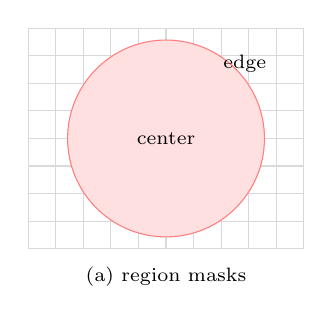
\begin{tikzpicture}[font=\scriptsize]
\draw[step=0.35, gray!30] (0,0) grid (3.5,2.8);
\draw[fill=blue!15, draw=blue!50] (1.75,1.4) circle (0.65);
\draw[fill=red!12, draw=red!50] (1.75,1.4) circle (1.25);
\node at (1.75,1.4) {center};
\node at (2.75,2.35) {edge};
\node at (1.75,-0.35) {(a) region masks};
\end{tikzpicture}
\end{subfigure}
\begin{subfigure}[t]{0.32\textwidth}
\centering
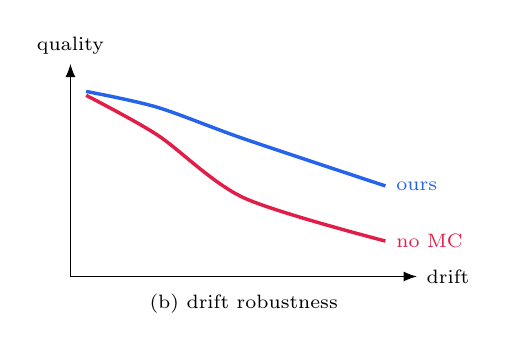
\begin{tikzpicture}[font=\scriptsize]
\draw[->] (0,0) -- (4.4,0) node[right] {drift};
\draw[->] (0,0) -- (0,2.7) node[above] {quality};
\draw[line width=1.25pt, dsdbRose] plot[smooth] coordinates {(0.2,2.3)(1.1,1.8)(2.2,1.0)(4.0,0.45)} node[right] {no MC};
\draw[line width=1.25pt, dsdbBlue] plot[smooth] coordinates {(0.2,2.35)(1.1,2.15)(2.2,1.75)(4.0,1.15)} node[right] {ours};
\node at (2.2,-0.35) {(b) drift robustness};
\end{tikzpicture}
\end{subfigure}
\begin{subfigure}[t]{0.32\textwidth}
\centering
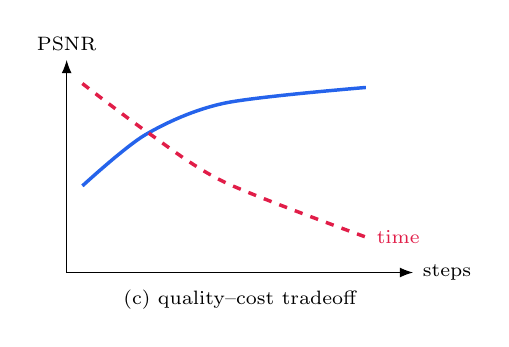
\begin{tikzpicture}[font=\scriptsize]
\draw[->] (0,0) -- (4.4,0) node[right] {steps};
\draw[->] (0,0) -- (0,2.7) node[above] {PSNR};
\draw[line width=1.25pt, dsdbBlue] plot[smooth] coordinates {(0.2,1.1)(1.0,1.75)(2.0,2.15)(3.8,2.35)};
\draw[line width=1.25pt, dashed, dsdbRose] plot[smooth] coordinates {(0.2,2.4)(1.0,1.8)(2.0,1.15)(3.8,0.45)} node[right] {time};
\node at (2.2,-0.35) {(c) quality--cost tradeoff};
\end{tikzpicture}
\end{subfigure}
\caption{Experiment evidence panels for region analysis, calibration-drift robustness, and quality--cost tradeoff. The schematic curves define the intended figure layout and are replaced by measured curves when experimental logs are available. The panels align visual evidence with the central claims: off-axis restoration, measurement-consistency robustness, and practical few-step inference.}
\label{fig:experiment_plan}
\end{figure*}

\subsection{State Diagnostics}
To show that $s_t$ is more than an attention map, the paper visualizes degradation states at early, middle, and late sampling stages. The maps are compared with reconstruction error, measurement residual, and field-dependent optical descriptors. A high correlation between $s_t$ and residual uncertainty, together with a monotonic decrease along the reverse trajectory, supports the interpretation of $s_t$ as a dynamic remaining-degradation state.

\subsection{Efficiency and Sampling Steps}
Diffusion restoration is often criticized for computational cost. The paper reports performance under different sampling budgets, such as 4, 8, 12, 20, and 50 steps. Runtime, memory, and parameter count are measured under a fixed hardware setting. This analysis is necessary to show whether the clean-domain anchor enables practical few-step restoration.

\section{Discussion}
The proposed method addresses the spatially nonuniform and dynamically evolving uncertainty of metalens photography. Its main advantage lies in separating three concepts that are often conflated in restoration diffusion models: the degraded measurement, the clean-domain anchor, and the remaining stochastic uncertainty. The fixed prior $\rho$ provides a physically meaningful forward uncertainty model, while the dynamic state $s_t$ controls the reverse process without invalidating the forward marginal.

Several limitations are acknowledged. First, the method relies on a usable approximation of the metalens forward operator. Severe calibration errors may reduce the reliability of measurement projection. Second, diffusion-bridge sampling is more expensive than single-pass deterministic restoration, although the clean-domain anchor allows the method to operate with relatively few sampling steps. Third, real paired metalens data may contain alignment errors, exposure mismatch, and reference-camera bias. These factors are handled with robust masks, measurement-consistency metrics, and unpaired real-image evaluation.

Future work may extend this framework toward joint optical design and reconstruction, adaptive calibration, raw-domain metalens restoration, and video metalens photography.

\section{Conclusion}
We presented a physics-anchored degradation-state diffusion bridge for metalens photography. The proposed framework treats metalens restoration as a field-dependent inverse problem with progressive spatial uncertainty. Instead of directly bridging from raw degraded measurements or relying on globally scheduled diffusion stochasticity, the method constructs a clean-domain anchor, estimates a fixed optical uncertainty prior, and uses a dynamic degradation state to modulate reverse stochastic transport. An explicit metalens measurement-consistency mechanism further constrains the restored image to explain the captured observation under the calibrated forward model. This formulation provides a principled and interpretable route for restoring metalens photographs under spatially nonuniform degradation, off-axis uncertainty, and calibration mismatch.

\appendices
\section{Implementation Checklist}
A reproducible implementation reports input resolution, sampling steps, backbone, optimizer, learning rate, weight decay, batch size, augmentation, PSF-bank interpolation, operator cache, and hardware. The logging protocol includes PSNR, SSIM, LPIPS, DISTS, measurement error, state correlation, off-axis metrics, runtime, and memory.

\section{Reviewer-Oriented Evidence Checklist}
Each central claim is connected to an observable piece of evidence:
\begin{itemize}
    \item Physics anchoring: report $\mathcal{E}_{\mathrm{meas}}=\|\hk(\hat x)-y\|_1$ and show residual maps.
    \item Dynamic state: report $\Corr(s_t,E_t)$ or $\Corr(s_t,M_t)$, state entropy, and temporal decay.
    \item Metalens specificity: report center, edge, off-axis, and chromatic-edge metrics.
    \item Calibration robustness: report PSF mismatch, field shift, chromatic perturbation, and noise mismatch curves.
    \item Practicality: report quality versus 4/8/12/20/50 sampling steps and runtime.
\end{itemize}

\section{Additional Figure Set}
The complete manuscript is organized around the following figure set:
\begin{itemize}
    \item Fig.~\ref{fig:overview}: overall pipeline: $\hk \rightarrow \mu/\rho \rightarrow s_t \rightarrow$ reverse bridge $\rightarrow$ measurement projection.
    \item Fig.~\ref{fig:concepts}: theoretical concept figure showing field-dependent PSF, dynamic state dissipation, and measurement projection.
    \item Fig.~\ref{fig:bridge_geometry}: bridge geometry contrasting generic diffusion, raw-observation bridging, and PA-DSDB.
    \item Fig.~\ref{fig:architecture}: module-level network architecture for one reverse step.
    \item Qualitative comparison on off-axis blur, chromatic leakage, ringing, and fine structures.
    \item Degradation-state diagnostics across early, middle, and late sampling steps.
    \item Calibration-drift robustness curves and sampling-step quality--cost curves.
\end{itemize}

\bibliographystyle{IEEEtran}
\bibliography{refs}

\end{document}
